%%%%%%%%%%%%%%%%%%%% BlackSheep.tex %%%%%%%%%%%%%%%%%%%%%%%%


% Packages %%%%%%%%%%%%%%%%%%%%%%%%%%%%%%%%%%%%%%%%%%%%%%%%%%%
\documentclass[graybox]{svmult}

\usepackage{mathptmx}      
%\usepackage{helvet} 
\usepackage[latin1]{inputenc}    % I want to see how it looks with this font    
%\usepackage{courier}       
\usepackage{type1cm}       
\usepackage{amsfonts}
\usepackage{makeidx}       
\usepackage{graphics}  
\usepackage{graphicx}     
\usepackage{subfigure}  
\usepackage{algorithm2e}
\usepackage{multicol}       
\usepackage[bottom]{footmisc}

\makeindex 

% New Commands
\newcommand{\PathSet}{\ensuremath{\mathcal P} }
\newcommand{\PathSetDistance}{\ensuremath{\mathcal G} }
\newcommand{\Z}{\mathbb{Z} }
\newcommand{\Path}{\ensuremath{P} }
\newcommand{\DCS}{\ensuremath{\Omega} }
\newcommand{\PathDistance}{\textsl{PD} }
\newcommand{\Q}{\textsl{Q} }

% Graph
\newcommand{\Graph}{\ensuremath{\mathcal G} }
\newcommand{\VertexSet}{\ensuremath{\mathcal V} }
\newcommand{\EdgeSet}{\ensuremath{\mathcal E} }

\newcommand{\MetricSpace}{\ensuremath{\mathcal M} }
\newcommand{\DistanceMetric}{\ensuremath{d_{min}} }

\newcommand{\Set}{\ensuremath{\textsl S} }
\newcommand{\VertexSetDistance}{\ensuremath{D_{VS}} }
\newcommand{\AddedDistance}{\ensuremath{D_{added}} }


% Title %%%%%%%%%%%%%%%%%%%%%%%%%%%%%%%%%%%%%%%%%%%%%%%%%%%%%%%%

\begin{document}

\title*{Bounded Diverse Paths and their application in Path Planning}
\author{Ana Huam\'an Quispe and Mike Stilman}
\institute{Center for Robotics and Intelligent Machines, Georgia Institute of Technology,Atlanta GA,\\ \email{ahuaman3@gatech.edu, mstilman@cc.gatech.edu}}

\maketitle

% Abstract %%%%%%%%%%%%%%%%%%%%%%%%%%%%%%%%%%%%%%%%%%%%%%%%%%%%%%%

\abstract{We present a formal definition of Bounded Diverse Paths and how this approach can be applied to Path Planning.\newline\indent
Our approach rests on principles of Digital Imagery as well as Optimal Control. We show its application to a practical problem, such as how to find diverse paths.}

%%%%%%%%%%%%%%%%%%%%%%%%%%%%%%%%%%%%%%%%%%%%%%%%%%%%%%%%%%%%%%%%
% Introduction
\section{Introduction}
\label{sec:Introduction}
Motion planning problems usually refer to the canonical problem of computing collision-free paths from a start to a goal position. Great efforts have been focused in developing techniques to produce \emph{optimal paths}, according to some cost metric. While this is useful in some scenarios, it is also true that there are situations in which it would be more useful to produce more than one possible path as a solution. We illustrate this better as an example:

Assume that you have a robotic arm such as in Fig.\ref{fig:IntroductionStartPosition} and you want to devise a path to reach the goal position in Fig.\ref{fig:IntroductionTargetPosition}. Say that you want to solve this problem by using \emph{search-based techniques} for high-dimensional spaces, such as \cite{Cohen2011AdaptivePrimitives}, which make use of a \emph{workspace heuristic of the end effector} to guide the configuration space search. If we use a standard optimal planner to obtain the optimal path in terms of length, we would get the green path depicted in Fig.\ref{fig:IntroductionPaths}. However, from Fig.\ref{fig:IntroductionTargetPosition}, it is easily seen that the path depicted in red would be more appropiate to describe what the real end effector path would look like. 

The red path would probably not be found by a standard planner since its longer than the optimal path. Hence, in this problem it makes sense for a planner to produce both paths and let the user decide which one is fit to the problem requirements. In order to produce both paths, we must establish that they are different in some way, or belong to \emph{different classes}.

% ...............................................
% Figure of Schunk and the End Effector Path
\begin{figure}[]
		\centering
		  \subfigure[Start Position]{
		   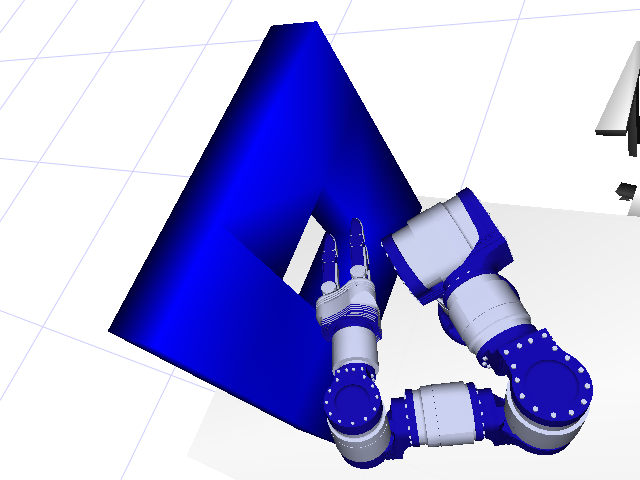
\includegraphics[width=0.4\textwidth]{figures/startPosition.png} 
		   \label{fig:IntroductionStartPosition}
          }
          \subfigure[Target position]{
	       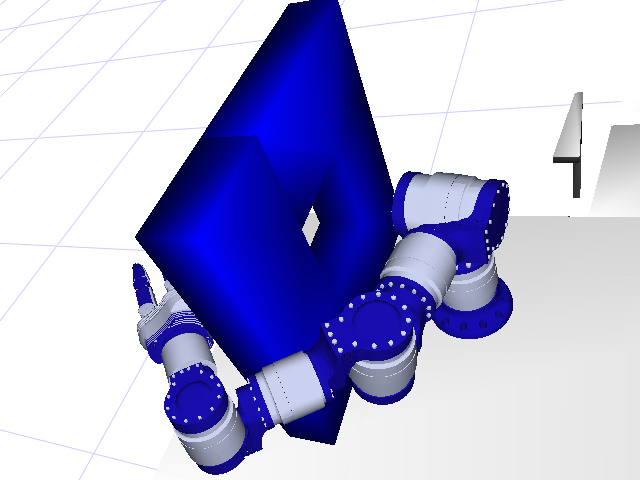
\includegraphics[width=0.4\textwidth]{figures/targetPosition.png} 	
	       \label{fig:IntroductionTargetPosition}
          }
		  \subfigure[Possible Paths]{
		   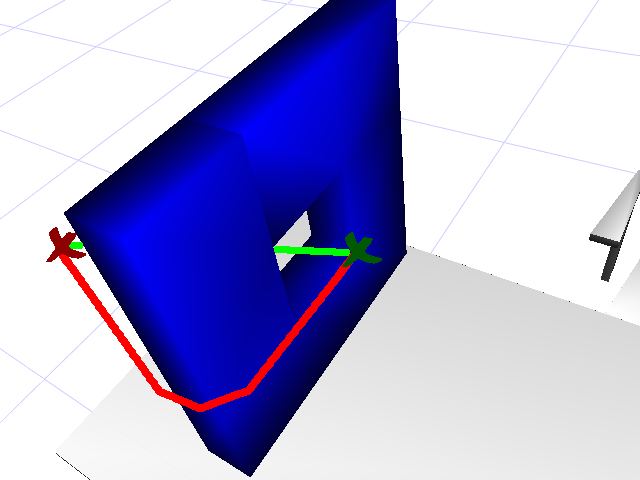
\includegraphics[width=0.4\textwidth]{figures/Torus3DEndingPointsDrawnX.png} 
		   \label{fig:IntroductionPaths}
          }          
          \caption{Application example: An optimal planner would find the green path, however the red one would be more useful}
          \label{fig:IntroductionHeuristic}
\end{figure}

\emph{Homotopy classes} are a straightforward concept to classify paths. Two paths are homotopic if one path can be continuously  deformed into another without passing through an obstacle. A homotopy class is a collection of homotopy paths. In two-dimensional environments, each obstacle generates at least a new homotopy class (ask Mike this) as it can be seen in the example at Fig.\ref{fig:IntroductionHomo2D}. 

% ...............................................
% Figure of Homotopy Paths in 2D
\begin{figure}[]
		\centering
		  \subfigure[Initial problem]{
		   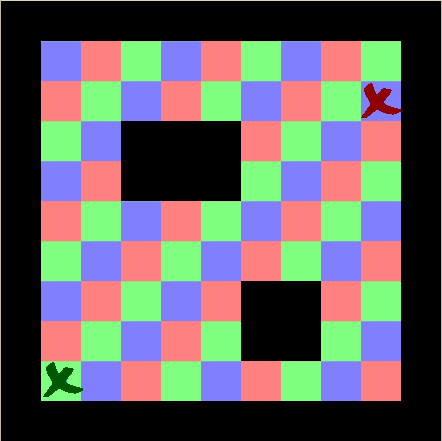
\includegraphics[width=0.3\textwidth]{figures/IntroductionHomo2Da.png} 
		   \label{fig:IntroductionHomo2Da}
          }
          \subfigure[Path in Homotopy class A]{
	       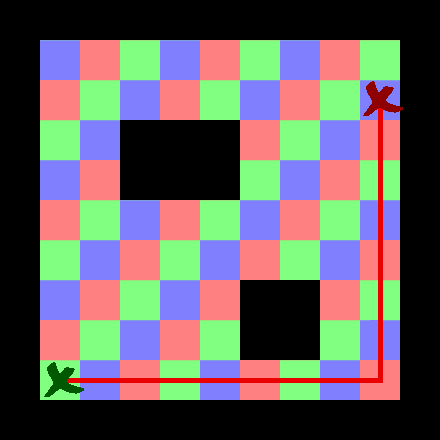
\includegraphics[width=0.3\textwidth]{figures/IntroductionHomo2Db_linee.png} 	
	       \label{fig:IntroductionHomo2Db}
          }
		  \subfigure[Path in Homotopy class B]{
		   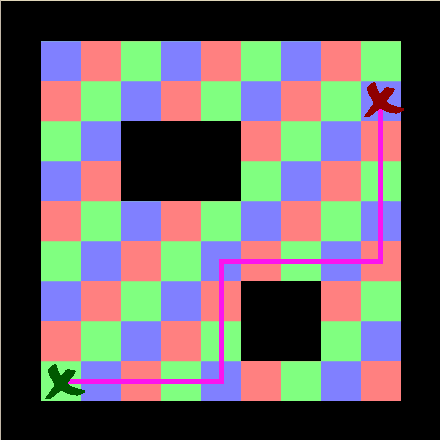
\includegraphics[width=0.3\textwidth]{figures/IntroductionHomo2Dc_linee.png} 
		   \label{fig:IntroductionHomo2Dc}
          }          
          \subfigure[Path in Homotopy class C]{
	       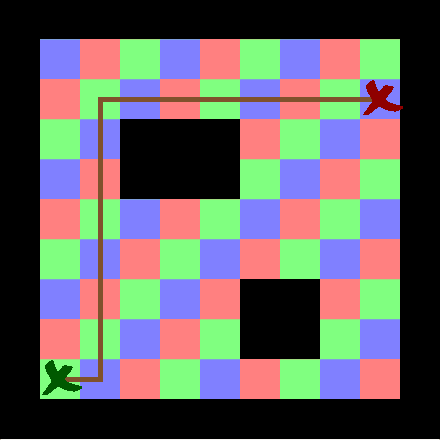
\includegraphics[width=0.3\textwidth]{figures/IntroductionHomo2Dd_linee.png} 	
	       \label{fig:IntroductionHomo2Dd}
          }
		  \subfigure[Path in Homotopy class D]{
		   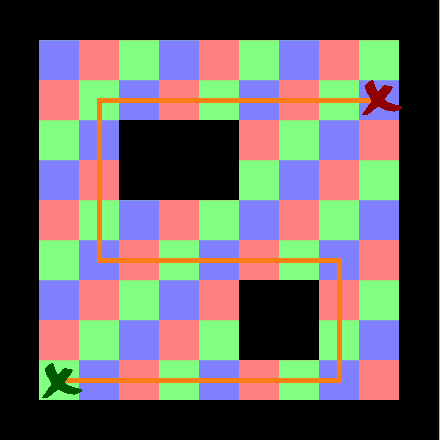
\includegraphics[width=0.3\textwidth]{figures/IntroductionHomo2De_linee.png} 
		   \label{fig:IntroductionHomo2De}
          }                   
          \caption{Homotopy classes in 2D environments}
          \label{fig:IntroductionHomo2D}
\end{figure}

In 3D environments, the specification of paths belonging to different homotopy classes is harder to determine, since only obstacles that contain \emph{holes} or obstacles stretching to infinity in two directions determine different homotopy classes (\cite{Bhattacharya2011Homotopy3D}). In Fig.\ref{fig:IntroductionHeuristic} the obstacle had one hole, so there were two homotopy classes, namely the set of paths that passed through the hole and the set that passed outside the obstacle. Now, think what would happen if the obstacle would have the shape shown in Fig.\ref{fig:IntroductionNoHomo3D}. The scenery is the same as in Fig. \ref{fig:IntroductionHeuristic}, with the exception that in Fig. \ref{fig:IntroductionNoHomo3D} the obstacle is not close-shaped anymore. Three paths are shown in Fig. \ref{fig:IntroductionNoHomo3DPaths}, all of them belonging to the same homotopic class. 

% .....................................................................................
% Example of Schunk in which Homotopic classification does not work as expected
\begin{figure}[]
		\centering
		  \subfigure[Problem proposed]{
		   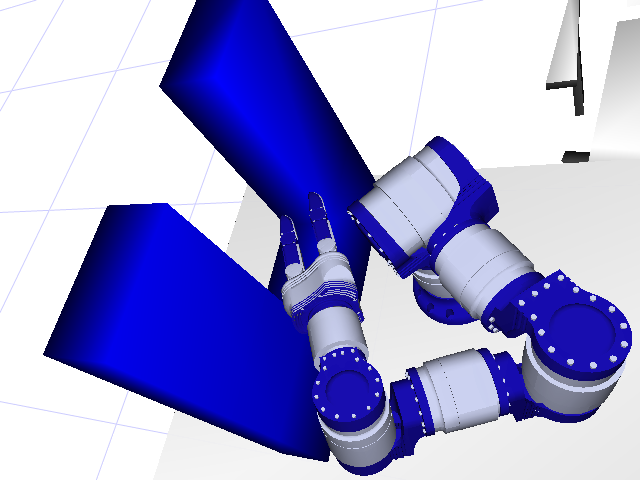
\includegraphics[width=0.4\textwidth]{figures/IntroductionNoHomo3D.png} 
		   \label{fig:IntroductionNoHomo3DProb}
          }
          \subfigure[Possible paths, all belonging to the same homotopic class]{
	       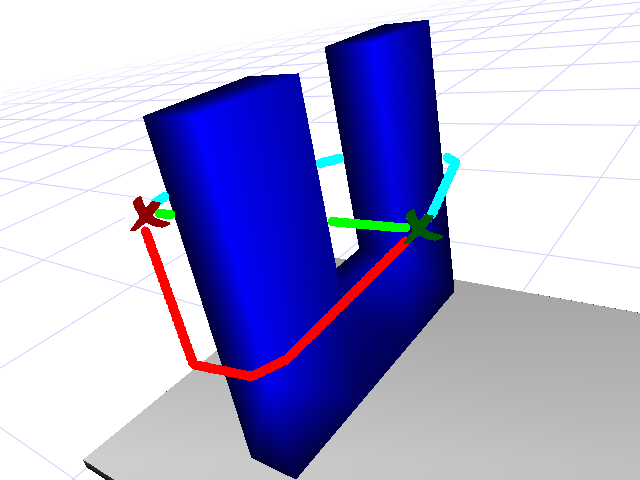
\includegraphics[width=0.4\textwidth]{figures/IntroductionNoHomo3DObstacleX.png} 	
	       \label{fig:IntroductionNoHomo3DPaths}
          }
          \caption{Application example: To classify the paths by their homotopy class is not very useful here}
          \label{fig:IntroductionNoHomo3D}
\end{figure}


From the example before, we see that describing paths based on their homotopy class is, for some cases, too strict and hence it does not help much in the generation of paths that are as \emph{diverse} as possible.

On this paper, we will propose a simple and intuitive method to automatically generate set of paths such that these are as \emph{diverse} as possible, making it possible to consider more than one alternative. 


%%%%%%%%%%%%%%%%%%%%%%%%%%%%%%%%%%%%%%%%%%%%%%%%%%%%%%%%%%%%%%%%
\section{Related Work}
\label{sec:RelatedWork}
Efforts to produce different paths have been mostly related to homotopy classification. The problem of homotopy in 2D environments has been throroughly studied and there are diverse solutions present in robotics literature. The approaches are diverse, ranging from geometric methods, such as \cite{}. Later on, Schmitzberger worked on the problem by using Probabilistic Roadmaps (\cite{Schmitzberger2002Homo2D}), obtaining a planner that was able to capture paths from different homotopy classes, however these paths were not optimal, due to the intrinsic randomized nature of the PRM.
\medskip
5
Bhattacharya et al presented an interesting method to find optimal paths with homotopic path constraints \cite{Bhattacharya2010Homotopy2D}, based on a weird rule that I still don't get but has something to do with my Electrical undergrad courses, for sure. Igarashi and Stilman (\cite{Igarashi2010Homotopy2D}) on the other hand, presented a simple and powerful algorithm that also generate optimal paths on different homotopy classes by using a variant of greedy search with a heuristic that build overlapping manifolds corresponding to the different homotopic classes.

Path generation with homotopic constraints in 3D environments has been recently studied in \cite{Bhattacharya2011Homotopy3D} by using more weird electrical laws that are extensive to any 3D scene (i.e. a 2D dynamic environment in which the time t is the third dimension).

As we saw in the introduction, Homotopy alone is not enough to get the variety we are looking for.
 
 
Here we can cite work of Likhachev et al \cite{Bhattacharya2011Homotopy3D}, and stuff about Distance Transform such as the work of Pedro Fzelnzab as well as the application of Distance Transforms to Path Planning, although its goal was different than ours

Mention coverage stuff by Zelinsky \cite{Zelinsky1993Coverage}

Problem pretty much solved by Stilman \cite{Igarashi2010Homotopy2D} and Likhachev \cite{Bhattacharya2010Homotopy2D}

Why it is hard and recent stuff from Knepper \cite{Knepper2012Equivalence} and roots from Simeon \cite{Simeon2000VisibilityPRM} and Jaillet \cite{Jaillet2008PathDeformation}

%%%%%%%%%%%%%%%%%%%%%%%%%%%%%%%%%%%%%%%%%%%%%%%%%%%%%%%%
\section{Definitions}
\label{sec:Definitions}

% ------------------------------------
% Search Space Definition
\begin{definition}[Search Space]
\label{def:SearchSpace}
We define a general \emph{search space} as an undirected connected graph $\Graph$, with a set \VertexSet of vertices and a set \EdgeSet of edges. In this paper, we further consider: 
\begin{itemize}
\item{\VertexSet: A finite path-connected set of discretized \emph{free} space locations (free voxels). $\VertexSet \in \mathbb{N}^{3}$ }
\item{\EdgeSet: A finite set of connections between two neighboring vertices $v_{i}, v_{j} \in \VertexSet$. }
\end{itemize} 
From the definition above, it is easy to see that occupied locations (i.e. obstacles) are not represented in \Graph. 
\end{definition}

Examples of Search Spaces are shown in Fig.\ref{fig:DiscreteSets}.  Fig.\ref{fig:PathConnectedSet} show a uniformly gridded box, where $\VertexSet$ is comprised of the free space voxels inside the colored grid. Fig.\ref{fig:ConnectedSet} shows a more complex space in which obstacles inside the box were added.

\begin{figure}[]
		\centering
		  \subfigure[Path Connected Set]{
		   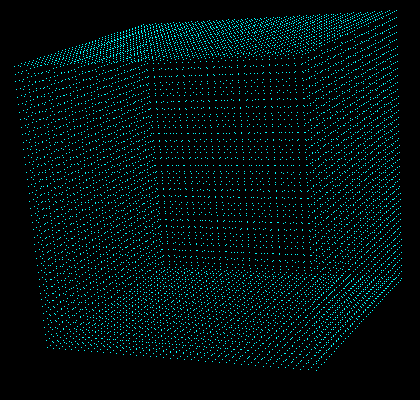
\includegraphics[width=0.4\textwidth]{figures/PathConnectedSet.png} 
		   \label{fig:PathConnectedSet}
          }
          \subfigure[Connected Set]{
	       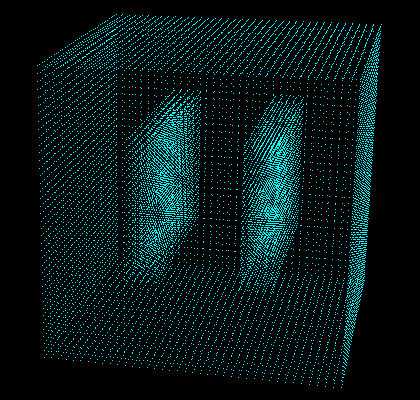
\includegraphics[width=0.4\textwidth]{figures/ConnectedSet.png} 	
	       \label{fig:ConnectedSet}
          }
          \caption{Examples of Discrete Connected Sets}
          \label{fig:DiscreteSets}
\end{figure}

% ---------------------------------------------
% Path
\begin{definition}[Path]
Given the set \VertexSet of vertices from \Graph and two vertices $v_{a}$ and $v_{b}$, we define a path \Path as a sequence of vertices such that:

\[ \Path = \{ p_{1}, p_{2},..., p_{n} \} \]

such that:
\begin{itemize}
\item{ $p_{1} = v_{a}$, $p_{n} = v_{b}$ }
\item{ $ (p_{i}, p_{i+1}) \in \EdgeSet, \forall p_{i} \in \Path$,  $i \in [1,n-1] $}
\end{itemize}

additionally, we define the cardinality of $\Path$: 
\[ \mid \Path \mid = n \]

\end{definition}
% ---------------------------------------------
% Metric Space
\begin{definition}[Metric Space]
\label{def:MetricSpace}
We define the \emph{metric space} \MetricSpace based on a given search space $\Graph$  as:
\begin{equation}
\MetricSpace = (\VertexSet, \DistanceMetric) 
\end{equation}

where 

\[ \DistanceMetric : \VertexSet \times \VertexSet \rightarrow \mathbb{R} \]

$\DistanceMetric$ is the length of the shortest path connecting any vertices $v_{i}$, $v_{j} \in \VertexSet$. $\DistanceMetric$ holds the following properties:

\begin{enumerate}
\item{$\DistanceMetric(x,y) \geq 0$ }
\item{$\DistanceMetric(x,y) = 0 \iff x = y$ }
\item{$\DistanceMetric(x,y) = \DistanceMetric(y,x)$ }
\item{$\DistanceMetric(x,z) \leq \DistanceMetric(x,y) + \DistanceMetric(y,z) $ }
\end{enumerate}
 
\end{definition}

% ---------------------------------------------------
% Definition Distance of a Vertex w.r.t. a Path Set
\begin{definition}[Vertex-Set Distance]
Consider a search space \Graph and its corresponding metric space $\MetricSpace$. Define a set of vertices $\Set$ as:

\[ \Set = \{ s_{1}, s_{2},...,s_{n_{s}} \},  s_{i} \in \VertexSet \]

The distance from any vertex $q \in \VertexSet$ with respect to \Set as the \emph{set distance} $\VertexSetDistance$ :
\[ \VertexSetDistance(q, S) = \inf_{ i = [ 1,..., n_{s} ] } \{ \DistanceMetric(q, s_{i}) \} \]
\end{definition}

% ------------------------------------------------
% Definition of Path Cost
\begin{definition}[Added Distance]
\label{def:AddedDistance}
Given a path $\Path \in \VertexSet$ and a set $\Set \in \VertexSet$. We define the \emph{added distance} ($\AddedDistance$) of $\Path$ with respect to $\Set$ as:

\[ \AddedDistance (\Path, \Set) = \sum _{i = 0}^{|\Path|} \VertexSetDistance(p_{i}, \Set) \]

\end{definition}

Based on Definition \ref{def:AddedDistance}, a special case occurs when the set $\Set$ is the union of a set of paths $\PathSet$:

\[ \PathSet = \bigcup_{i = 1}^{k} \Path_{k} = \Path_{1} \cup \Path_{2} \cup ... \cup \Path_{k} \] 

Then, the Added Distance from a path $P_{k+1}$ with respect to this set of paths $\PathSet$ is:

\begin{equation} 
\AddedDistance (\Path_{k+1}, \PathSet) =  \sum _{i = 0}^{|\Path_{k+1}|} \VertexSetDistance({p_{k+1}}_{i}, \PathSet) 
\label{eq:PathDistance}
\end{equation}

Now we have all the needed definitions to formally enunciate our problem:

% .....................................................
% Problem Definition
\begin{definition}[Diverse Paths Problem]
\label{def:DiversePathProblem}
For a search space \Graph we define a start and target locations, represented by the vertices $v_{start}$ and $v_{target} \in \VertexSet$.  We want to find a set of paths $\PathSet$ that hold the following conditions:

\begin{itemize}
\item{$\PathSet$ must always contain the shortest path from $v_{start}$ to $v_{target}$ ($\Path^{*}$)  }
\item{The paths belonging to $\PathSet$ must be bounded in length with respect to $\Path^{*}$. Formally:
\begin{equation} 
\forall \Path_{i} \in \PathSet, \left | \Path_{i} \right | \leq \alpha \left| \Path^{*} \right |, \alpha \geq 1 
\label{eq:LengthBound}
\end{equation}

This condition allows to avoid considering paths excessively long}
\item{The added distance $\AddedDistance$ between a path $\Path_{i}$ and $\PathSet \setminus \Path_{i}$ (the remaining paths in $\PathSet$) is a maximum. Meaning, there is \textbf{no other path} that can have a greater $\AddedDistance$ than $\Path_{i}$ (and that simultaneously holds the condition in (\ref{eq:LengthBound}) }
\end{itemize}
\end{definition}

In the next section, we present an algorithm to systematically build $\PathSet$.

%%%%%%%%%%%%%%%%%%%%%%%%%%%%%%%%%%%%%%%%%%%%%%%%%%%%%%%%%%%%%
% Section
\section{Algorithm}
Let us formulate the problem as an \emph{optimization problem}, and then we will intuitively derive the algorithm presented.

From Definition \ref{DiversePathProblem}, we observe that our goal is to obtain a \emph{sequence} of paths, in which $\Path_{i+1}$ has a relationship with respect to the \emph{previous paths} ( $\Path_{1}$, $\Path_{2}$,...,$\Path_{i}$ ). Hence, we can formulate the problem by solving it sequentially.
\medskip

Now, our premise is that $\Path_{i+1}$ must maximize the distance between itself and the other previous paths. So, we can say that we want to maximize this expression:

\[ \Path_{i+1} = \argmax _{\forall \Path \in Q} f(\Path) = \AddedDistance (\Path, \PathSet) \]

\begin{algorithm}

\end{algorithm}

\bibliographystyle{plain}
\bibliography{references}

\end{document}
